\documentclass[a4paper,fleqn]{cas-dc}
\usepackage[numbers]{natbib}
\usepackage{siunitx}
\usepackage{amsmath}
\usepackage{booktabs}
\usepackage{graphicx}

% Every number quoted in the prose is generated by
% experiments/exp_06_unstable_saddle_and_fouling.py
% Generated by experiments/exp_06_unstable_saddle_and_fouling.py
\newcommand{\TfNom}{350}
\newcommand{\TfSad}{320}
\newcommand{\Tjf}{300}
\newcommand{\umax}{300}
\newcommand{\slew}{80}
\newcommand{\dtCtrl}{0.02}
\newcommand{\qjNom}{100.00}
\newcommand{\kappaFoul}{0.10}
\newcommand{\uaMin}{30}
\newcommand{\bandRun}{5}
\newcommand{\tShock}{2}
\newcommand{\tauCsiso}{0.10}
\newcommand{\horizonShock}{60}
\newcommand{\horizonFoul}{80}
\newcommand{\TNom}{396.65}
\newcommand{\CaNom}{0.0502}
\newcommand{\TjNom}{348.33}
\newcommand{\lamANom}{-1.5712}
\newcommand{\lamBNom}{-11.8006}
\newcommand{\lamCNom}{-13.2693}
\newcommand{\fcritNom}{60.0}
\newcommand{\rANom}{0.9498}
\newcommand{\nBranchNom}{1}
\newcommand{\convNom}{95.0}
\newcommand{\TSad}{345.00}
\newcommand{\CaSad}{0.5896}
\newcommand{\TjSad}{328.96}
\newcommand{\qjSad}{55.38}
\newcommand{\lamASad}{0.7435}
\newcommand{\lamBSad}{-0.9031}
\newcommand{\lamCSad}{-8.2884}
\newcommand{\fcritSad}{40.4}
\newcommand{\rASad}{0.4104}
\newcommand{\nBranchSad}{3}
\newcommand{\convSad}{41.0}
\newcommand{\TlowSad}{322.65}
\newcommand{\ThighSad}{378.97}
\newcommand{\lamLow}{-0.613}
\newcommand{\lamHigh}{-2.225}
\newcommand{\tauU}{1.345}
\newcommand{\qMultiLo}{36.3}
\newcommand{\qMultiHi}{80.3}
\newcommand{\nNomUnstable}{0}
\newcommand{\QrMaxFull}{5.957}
\newcommand{\TjMinFull}{324.16}
\newcommand{\QrMaxSixty}{4.749}
\newcommand{\TjMinSixty}{316.11}
\newcommand{\QrMaxFiftyFive}{4.579}
\newcommand{\TjMinFiftyFive}{314.97}
\newcommand{\QgNom}{4.749}
\newcommand{\nPortrait}{36}
\newcommand{\nIgnite}{17}
\newcommand{\kU}{-0.4413}
\newcommand{\tauUmodel}{1.345}
\newcommand{\thetaU}{0.648}
\newcommand{\boundU}{0.697}
\newcommand{\Tzero}{0.590}
\newcommand{\tcMaxPI}{0.293}
\newcommand{\KcSiso}{-4.073}
\newcommand{\TiSiso}{2.993}
\newcommand{\Ktwo}{-0.1864}
\newcommand{\tauTwo}{0.1287}
\newcommand{\KcSlave}{-4.643}
\newcommand{\TiSlave}{0.1287}
\newcommand{\KoneFit}{4.696}
\newcommand{\tauOneFit}{0.887}
\newcommand{\thetaOneFit}{0.816}
\newcommand{\KcMaster}{0.116}
\newcommand{\TiMaster}{0.887}
\newcommand{\absSiso}{-0.064}
\newcommand{\absCasc}{-0.119}
\newcommand{\absInner}{-0.271}
\newcommand{\ffSad}{84.58}
\newcommand{\GzeroNom}{-0.1957}
\newcommand{\KtwoNom}{-0.2416}
\newcommand{\ratioNom}{0.810}
\newcommand{\KoneNom}{0.576}
\newcommand{\detNom}{34.564}
\newcommand{\traceNom}{-16.641}
\newcommand{\absANom}{-2.433}
\newcommand{\gainErrNom}{40.5}
\newcommand{\GzeroSad}{0.4413}
\newcommand{\KtwoSad}{-0.1864}
\newcommand{\ratioSad}{-2.367}
\newcommand{\KoneSad}{4.521}
\newcommand{\detSad}{0.375}
\newcommand{\traceSad}{-0.679}
\newcommand{\absASad}{-0.340}
\newcommand{\gainErrSad}{-152.4}
\newcommand{\qjShockTjf}{84.58}
\newcommand{\bThreeShockTjf}{-0.948}
\newcommand{\absShockTjfSiso}{0.055}
\newcommand{\absShockTjfCascade}{-0.059}
\newcommand{\qjShockTf}{87.80}
\newcommand{\bThreeShockTf}{-1.198}
\newcommand{\absShockTfSiso}{-0.016}
\newcommand{\absShockTfCascade}{-0.091}
\newcommand{\iaeTjfSiso}{497.11}
\newcommand{\peakTjfSiso}{19.33}
\newcommand{\tvTjfSiso}{1561.7}
\newcommand{\qmaxTjfSiso}{177.3}
\newcommand{\ptpTjfSiso}{30.46}
\newcommand{\iaeTjfCascade}{23.28}
\newcommand{\peakTjfCascade}{1.83}
\newcommand{\tvTjfCascade}{152.9}
\newcommand{\qmaxTjfCascade}{97.7}
\newcommand{\ptpTjfCascade}{0.36}
\newcommand{\iaeTjfCascadeff}{12.89}
\newcommand{\peakTjfCascadeff}{1.01}
\newcommand{\tvTjfCascadeff}{96.4}
\newcommand{\qmaxTjfCascadeff}{91.6}
\newcommand{\ptpTjfCascadeff}{0.21}
\newcommand{\iaeTfSiso}{230.03}
\newcommand{\peakTfSiso}{19.24}
\newcommand{\tvTfSiso}{740.8}
\newcommand{\qmaxTfSiso}{167.6}
\newcommand{\ptpTfSiso}{8.34}
\newcommand{\iaeTfCascade}{132.07}
\newcommand{\peakTfCascade}{24.82}
\newcommand{\tvTfCascade}{584.4}
\newcommand{\qmaxTfCascade}{190.0}
\newcommand{\ptpTfCascade}{0.84}
\newcommand{\iaeTfCascadeff}{132.07}
\newcommand{\peakTfCascadeff}{24.82}
\newcommand{\tvTfCascadeff}{584.4}
\newcommand{\qmaxTfCascadeff}{190.0}
\newcommand{\ptpTfCascadeff}{0.84}
\newcommand{\iaeRedTjf}{95.3}
\newcommand{\iaeRedTf}{42.6}
\newcommand{\iaeRedFF}{44.6}
\newcommand{\fstabSiso}{89.3}
\newcommand{\qstabSiso}{59.3}
\newcommand{\fstabCascade}{86.1}
\newcommand{\qstabCascade}{60.8}
\newcommand{\bThreeNom}{-1.448}
\newcommand{\bThreeCrit}{-0.315}
\newcommand{\bThreeRatio}{4.6}
\newcommand{\tsatNomSiso}{10.02}
\newcommand{\trunNomSiso}{13.18}
\newcommand{\TendNomSiso}{416.40}
\newcommand{\uaSatNomSiso}{57.0}
\newcommand{\tsatNomCascade}{9.26}
\newcommand{\trunNomCascade}{13.18}
\newcommand{\TendNomCascade}{416.40}
\newcommand{\uaSatNomCascade}{59.0}
\newcommand{\tpredNom}{8.92}
\newcommand{\tsatSadSiso}{32.32}
\newcommand{\trunSadSiso}{28.06}
\newcommand{\TendSadSiso}{387.87}
\newcommand{\uaSatSadSiso}{44.8}
\newcommand{\tsatSadCascade}{33.06}
\newcommand{\trunSadCascade}{4.06}
\newcommand{\TendSadCascade}{387.88}
\newcommand{\uaSatSadCascade}{43.3}
\newcommand{\tpredSad}{46.36}


\shorttitle{Thermal controllability limits and cascade control in exothermic CSTRs}
\shortauthors{G.M. de Andrade and E.R. Edwards}

\begin{document}
\let\WriteBookmarks\relax
\def\floatpagepagefraction{1}
\def\textpagefraction{.001}

\title [mode = title]{Thermal Controllability Limits and Cascade Control in Exothermic CSTRs under Cooling Capacity Degradation}

\author[1]{Gabriel Marques de Andrade}[orcid=]
\cormark[1]
\ead{gmandrade.egm@uesc.br}
\credit{Conceptualization, Software, Methodology, Investigation, Writing -- original draft}

\author[1]{Elilton Rodrigues Edwards}
\ead{eredwards@uesc.br}
\credit{Supervision, Methodology, Writing -- review \& editing}

\affiliation[1]{organization={Department of Exact and Technological Sciences (DCET), State University of Santa Cruz (UESC)},
    addressline={Rodovia Jorge Amado, km 16},
    city={Ilh\'eus},
    postcode={45662-900},
    state={Bahia},
    country={Brazil}}

\cortext[1]{Corresponding author}

\begin{abstract}
Exothermic continuous stirred tank reactors are often said to be hard to control because they may operate at open-loop unstable steady states, yet the instability, the actuator limits and the loss of heat-transfer capacity are rarely separated. This work separates them on a three-state reactor--jacket model with a coolant valve limited in amplitude and slew rate. With the nominal feed the heat balance has one stable root for every admissible coolant flow, so an unstable steady state exists only when the feed is cooled; at $T_f=\TfSad$~K the middle branch at $\TSad$~K is a saddle with $\lambda_1=+\lamASad$~min$^{-1}$. A single-loop SIMC controller stabilizes this saddle only for closed-loop time constants below $\tcMaxPI$~min, whereas the classical bound $\tau_c<\tau_u-\theta$ is exact only for proportional action. A sequential cascade works because tight jacket regulation leaves the stable concentration--temperature sub-block; the open-loop gain ratio used to tune the master loop then has the wrong sign. Against a $+10$~K coolant shock the cascade reduces the integral absolute error by $\iaeRedTjf\%$ and static utility feedforward by a further $\iaeRedFF\%$, while the single loop falls into a limit cycle. Under reaction-driven fouling, fixed-gain loops lose the saddle at $UA\approx\fstabCascade$--$\fstabSiso\%$ of its clean value, well before the thermodynamic limit at $\fcritSad\%$, because fouling shrinks the actuator gain.
\end{abstract}


\begin{highlights}
\item The benchmark CSTR has a single stable steady state unless the feed is cooled.
\item Tight jacket regulation turns the open-loop unstable saddle into a stable plant.
\item Open-loop gain ratios misjudge the master gain and flip its sign at the saddle.
\item Fouling shrinks actuator gain; fixed-gain loops fail before the cooling limit.
\end{highlights}


\begin{keywords}
Exothermic CSTR \sep Open-loop instability \sep Cascade control \sep SIMC tuning \sep Jacket fouling \sep Thermal runaway
\end{keywords}

\maketitle

\section{Introduction}
\label{sec:introduction}

The thermal behaviour of an exothermic continuous stirred tank reactor (CSTR) is set by the competition between heat generation, which grows exponentially with temperature through the Arrhenius law, and heat removal, which grows at most linearly. Since the work of Aris and Amundson \cite{aris1958analysis} and Uppal, Ray and Poore \cite{uppal1974dynamic} this competition is known to produce multiple steady states, open-loop unstable middle branches, limit cycles and parametric sensitivity. The textbook treatment of reactor control \cite{seborg2010process,bequette2003process,luyben2007chemical} adds two practical facts: the coolant valve has finite stroke and finite speed, and the heat-transfer coefficient of the jacket decays during operation because of fouling. In industrial practice the reactor temperature is regulated by a cascade, in which a master loop on the reactor temperature sets the jacket temperature and a slave loop moves the coolant valve \cite{shinskey1996process,seborg2010process}.

These three ingredients---open-loop instability, actuator limits and loss of cooling capacity---are usually discussed together under the label ``thermal runaway''. They are, however, different mechanisms with different remedies. An open-loop unstable operating point can be stabilized by feedback if the controller is fast enough and the actuator has authority; a saturated actuator cannot be helped by any control law; and a degraded heat exchanger changes the plant seen by a fixed-gain controller long before it removes the steady state. A controllability study must therefore say which of these limits is active, and where.

This paper makes that separation on a well-documented three-state benchmark: a first-order irreversible exothermic reaction in a CSTR with a dynamic cooling jacket, the same model used in our companion studies of PID tuning and predictive control. Three questions are addressed:
\begin{enumerate}
    \item Does the benchmark actually have an open-loop unstable steady state, and where? We find that with the nominal feed temperature it does not; steady-state multiplicity appears only when the feed is cooled. All results on the unstable saddle are therefore obtained at a cooled feed, $T_f=\TfSad$~K, and stated as such.
    \item How should a single-loop and a cascade controller be tuned on the saddle, and why does the cascade work? We combine the simple internal model control (SIMC) rules \cite{skogestad2003simple} with an exact analysis of the closed-inner-loop dynamics, and show that the open-loop gain ratio commonly used for the master design can have the wrong sign at an unstable point.
    \item What happens when the heat-transfer coefficient decays continuously? We introduce a fouling law driven by the reaction rate and compare the time at which the valve saturates with a closed-form quasi-steady prediction. At the stable nominal point the prediction holds; at the saddle the fixed-gain loops are lost much earlier, for a reason that has nothing to do with the cooling capacity.
\end{enumerate}

The contributions are the following. (i) A map of the steady-state branches of the benchmark versus coolant flow and feed temperature, with a closed-form expression for the critical heat-transfer capacity below which a temperature setpoint cannot be held with the valve fully open. (ii) A derivation showing that the condition $\tau_c<\tau_u-\theta$ for an unstable first-order-plus-delay model---a form of the requirement that the closed loop be faster than the unstable pole \cite{stein2003respect}---is exact for proportional control of this reactor but not sufficient once the SIMC integral time is added. (iii) The exact static gain of the master loop from the concentration--temperature sub-block of the Jacobian, and its comparison with the open-loop ratio approximation. (iv) A reaction-driven fouling model, a time-to-saturation formula, and the observation that fouling destabilizes fixed-gain loops on the saddle because it shrinks the actuator gain of the coolant valve. All numbers in the paper are generated by one script and are traceable to CSV files.

Section~\ref{sec:model} presents the model, the multiplicity analysis and the thermodynamic limit. Section~\ref{sec:design} derives the controllers. Section~\ref{sec:fouling} introduces the fouling model. Section~\ref{sec:results} reports the simulations and Section~\ref{sec:conclusion} concludes.

\section{Process model, multiplicity and the thermodynamic limit}
\label{sec:model}

\subsection{Reactor--jacket model and actuator}
The reactor hosts the irreversible first-order reaction $A\rightarrow B$ with rate $r_A=k_0\,e^{-E/(RT)}C_A$. With constant volumes and physical properties, the mass balance of $A$ and the energy balances of the reactor and of the jacket are
\begin{align}
\frac{dC_A}{dt} &= \frac{q}{V}\left(C_{Af}-C_A\right) - r_A, \label{eq:mass}\\
\frac{dT}{dt} &= \frac{q}{V}\left(T_f-T\right) + \frac{-\Delta H}{\rho c_p}\,r_A - \frac{UA}{V\rho c_p}\left(T-T_j\right), \label{eq:energy}\\
\frac{dT_j}{dt} &= \frac{q_j}{V_j}\left(T_{jf}-T_j\right) + \frac{UA}{V_j\rho_j c_{pj}}\left(T-T_j\right). \label{eq:jacket}
\end{align}
The manipulated variable is the coolant flow $q_j$; the measured outputs are $T$ and $T_j$. The valve is limited to $q_j\in[0,\umax]$~L/min and to a slew rate of $\slew$~L/min$^2$, and the controllers run with a zero-order hold at $\Delta t=\dtCtrl$~min. Table~\ref{tab:parameters} lists the parameters. The heat-transfer capacity $UA$ enters Eqs.~\eqref{eq:energy}--\eqref{eq:jacket} as a time-varying input, which is how fouling is introduced in Section~\ref{sec:fouling}; all other parameters are constant except where a disturbance is stated.

\begin{table*}[t]
\centering
\footnotesize
\caption{Model, actuator and sampling parameters.}
\label{tab:parameters}
\resizebox{\ifdim\width>\textwidth\textwidth\else\width\fi}{!}{%
\begin{tabular}{lc}
\toprule
Symbol & Value \\
\midrule
$q$, $V$, $V_j$ & 100 L/min, 100 L, 20 L \\
$k_0$, $E/R$ & 7.2e+10 min$^{-1}$, 8750 K \\
$-\Delta H$ & 5.0e+04 cal/mol \\
$\rho c_p$, $\rho_j c_{pj}$ & 500, 500 cal/(L K) \\
$UA_0$ & 5.0e+04 cal/(min K) \\
$C_{Af}$, $T_{jf}$ & 1.0 mol/L, 300 K \\
$T_f$ (nominal / cooled) & 350 / 320 K \\
$[u_{\min}, u_{\max}]$, slew & [0, 300] L/min, 80 L/min$^2$ \\
$\Delta t$ & 0.02 min \\
\bottomrule
\end{tabular}%
}
\end{table*}


Linearizing Eqs.~\eqref{eq:mass}--\eqref{eq:jacket} at an equilibrium $(\bar C_A,\bar T,\bar T_j,\bar q_j)$ gives $\dot{\mathbf{x}}=\mathbf{A}\mathbf{x}+\mathbf{b}\,q_j$ with
\begin{equation}
\mathbf{A}=\begin{bmatrix} a_{11} & a_{12} & 0\\ a_{21} & a_{22} & a_{23}\\ 0 & a_{32} & a_{33}\end{bmatrix},\qquad
\mathbf{b}=\begin{bmatrix}0\\0\\ b_3\end{bmatrix},\qquad b_3=\frac{T_{jf}-\bar T_j}{V_j}.
\label{eq:jacobian}
\end{equation}
The input enters only through the jacket, and its gain $b_3$ is proportional to the temperature difference between the coolant supply and the jacket. This structural fact will matter twice: for the cascade, whose slave loop acts on exactly this channel, and for fouling, which drives $\bar T_j$ towards $T_{jf}$ and therefore $b_3$ towards zero. The transfer function from $q_j$ to $T$ follows from Eq.~\eqref{eq:jacobian} as
\begin{equation}
G(s)=\frac{b_3\,a_{23}\,(s-a_{11})}{\det(s\mathbf{I}-\mathbf{A})},
\label{eq:gs}
\end{equation}
with a single zero at $s=a_{11}<0$.

\subsection{Van Heerden analysis and steady-state branches}
At steady state, the mass and jacket balances give
\begin{gather}
C_A(T)=\frac{qC_{Af}}{q+Vk(T)},\\
T_j(T,q_j)=\frac{q_jT_{jf}+(UA/\rho_jc_{pj})\,T}{q_j+UA/\rho_jc_{pj}}.
\end{gather}
Equilibria are the intersections of the heat generation and removal curves \cite{aris1958analysis,uppal1974dynamic}
\begin{align}
Q_g(T) &= (-\Delta H)\,V\,k(T)\,C_A(T), \label{eq:qg}\\
Q_r(T,q_j) &= q\rho c_p\,(T-T_f) + UA\,\bigl(T-T_j(T,q_j)\bigr). \label{eq:qr}
\end{align}
An intersection at which $\partial Q_g/\partial T>\partial Q_r/\partial T$ violates the Van Heerden slope condition and is open-loop unstable \cite{seborg2010process,bequette2003process}; the converse is necessary but not sufficient, so stability is always checked here on the spectrum of $\mathbf{A}$.

Figure~\ref{fig:van_heerden}(b) shows the equilibrium temperature versus coolant flow, computed by bracketing every sign change of $Q_g-Q_r$ on a fine temperature grid and refining it with Brent's method. With the nominal feed temperature, $T_f=\TfNom$~K, the curve is single-valued: over the whole valve range there is one equilibrium, and none of the sampled equilibria has an eigenvalue with positive real part (count of unstable points: $\nNomUnstable$). At the nominal flow of $\qjNom$~L/min the reactor sits at $\TNom$~K with $\convNom\%$ conversion and eigenvalues $\lamANom$, $\lamBNom$ and $\lamCNom$~min$^{-1}$.

Cooling the feed moves the generation curve with respect to the removal line. At $T_f=\TfSad$~K three equilibria coexist on the sampled grid for $q_j$ between $\qMultiLo$ and $\qMultiHi$~L/min. Placing the middle branch at $\bar T=\TSad$~K fixes $\bar C_A$ from the mass balance, $\bar T_j$ from Eq.~\eqref{eq:energy} and then $\bar q_j=\qjSad$~L/min from Eq.~\eqref{eq:jacket}; Powell's hybrid root finder started from this point returns it to machine precision. The three equilibria at this flow are listed in Table~\ref{tab:operating_points}: an extinguished state at $\TlowSad$~K (largest eigenvalue real part $\lamLow$~min$^{-1}$), the middle state at $\TSad$~K, and an ignited state at $\ThighSad$~K ($\lamHigh$~min$^{-1}$). The middle state has eigenvalues $+\lamASad$, $\lamBSad$ and $\lamCSad$~min$^{-1}$: one unstable direction, i.e.\ a saddle, with an unstable time constant $\tau_u=1/\lambda_1=\tauU$~min. Its conversion is $\convSad\%$, against $\convNom\%$ at the nominal point.

\begin{figure*}[t]
\centering
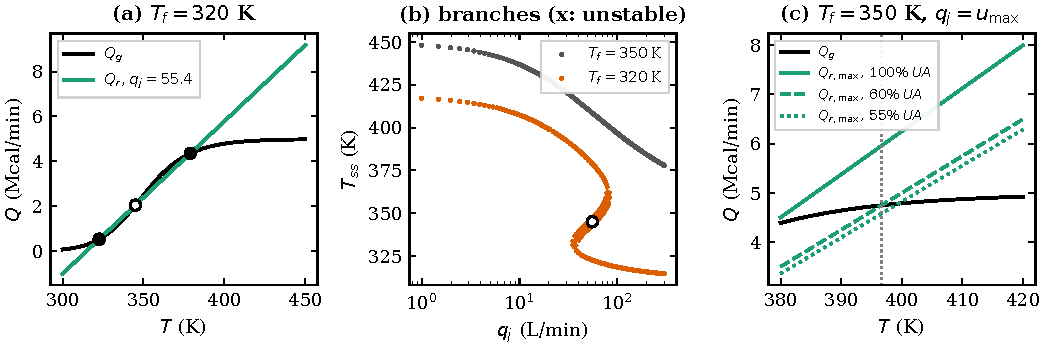
\includegraphics[width=\textwidth]{figures/fig1_van_heerden.pdf}
\caption{(a) Heat generation and removal at the saddle flow $q_j=\qjSad$~L/min and $T_f=\TfSad$~K; open marker: unstable equilibrium. (b) Equilibrium temperature versus coolant flow for the nominal and the cooled feed; crosses: open-loop unstable equilibria. (c) Heat generation and maximum heat removal ($q_j=u_{\max}$) at the nominal feed for three levels of $UA$; dotted line: nominal setpoint.}
\label{fig:van_heerden}
\end{figure*}

\begin{table*}[t]
\centering
\footnotesize
\caption{Operating points. Equilibria: number of steady states at the same $q_j$; $UA_{\mathrm{crit}}$: heat-transfer capacity below which holding $T$ needs $q_j > u_{\max}$ (Eq.~\eqref{eq:ua_crit}).}
\label{tab:operating_points}
\resizebox{\ifdim\width>\textwidth\textwidth\else\width\fi}{!}{%
\begin{tabular}{lcccccccc}
\toprule
Point & $T_f$ (K) & $q_j$ (L/min) & $T$ (K) & $C_A$ (mol/L) & $T_j$ (K) & $\lambda_{1,2,3}$ (min$^{-1}$) & Equilibria & $UA_{\mathrm{crit}}/UA_0$ (\%) \\
\midrule
Nominal & 350 & 100.00 & 396.65 & 0.0502 & 348.33 & -1.571, -11.801, -13.269 & 1 & 60.0 \\
Saddle & 320 & 55.38 & 345.00 & 0.5896 & 328.96 & 0.744, -0.903, -8.288 & 3 & 40.4 \\
\bottomrule
\end{tabular}%
}
\end{table*}


The open-loop phase portrait at the saddle flow, Fig.~\ref{fig:phase_portrait}, shows the separatrix behaviour reported by Uppal, Ray and Poore \cite{uppal1974dynamic}: of $\nPortrait$ initial conditions on a grid in the $(C_A,T)$ plane, $\nIgnite$ end on the ignited branch and the rest on the extinguished branch. A reactor operated at $\TSad$~K without feedback leaves the setpoint in either direction depending on the sign of the first perturbation, so any loss of feedback authority produces either ignition or extinction.

\begin{figure}[t]
\centering
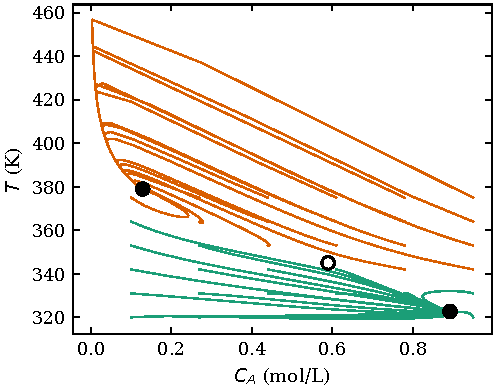
\includegraphics[width=\columnwidth]{figures/fig2_phase_portrait.pdf}
\caption{Open-loop trajectories at $q_j=\qjSad$~L/min, $T_f=\TfSad$~K, projected on the $(C_A,T)$ plane over 20~min. Orange: trajectories ending on the ignited branch; green: on the extinguished branch. Open marker: saddle at $\TSad$~K.}
\label{fig:phase_portrait}
\end{figure}

\subsection{Thermodynamic controllability limit}
Feedback can move an equilibrium but cannot create cooling capacity. If the temperature and the concentration are held at their setpoint values, the heat that must leave through the wall,
\begin{equation}
Q_{\mathrm{load}} = V\rho c_p\left[\frac{q}{V}\left(T_f-\bar T\right)+\frac{-\Delta H}{\rho c_p}\,r_A(\bar C_A,\bar T)\right],
\end{equation}
does not depend on $UA$. The jacket temperature that removes it is $\bar T_j=\bar T-Q_{\mathrm{load}}/UA$, and the jacket balance then gives the required flow $q_j=Q_{\mathrm{load}}/\left[\rho_jc_{pj}(\bar T_j-T_{jf})\right]$. Setting $q_j=u_{\max}$ yields the critical heat-transfer capacity
\begin{equation}
UA_{\mathrm{crit}} = \frac{Q_{\mathrm{load}}}{\bar T - T_{jf} - Q_{\mathrm{load}}/(\rho_jc_{pj}\,u_{\max})},
\label{eq:ua_crit}
\end{equation}
below which no controller acting on this valve can hold the setpoint. Equivalently, $UA<UA_{\mathrm{crit}}$ is the condition $Q_g(\bar T)>Q_{r,\max}(\bar T)$, with $Q_{r,\max}(T)=Q_r(T,u_{\max})$.

At the nominal point Eq.~\eqref{eq:ua_crit} gives $UA_{\mathrm{crit}}=\fcritNom\%$ of the clean value. The heat generated at the setpoint is $Q_g=\QgNom$~Mcal/min. With a clean jacket and the valve fully open the reactor could remove $Q_{r,\max}=\QrMaxFull$~Mcal/min; at $60\%\,UA$ the maximum removal is $\QrMaxSixty$~Mcal/min, equal to the generation within the printed precision, so $60\%$ is the boundary itself; at $55\%\,UA$ it drops to $\QrMaxFiftyFive$~Mcal/min, below $Q_g$. Figure~\ref{fig:van_heerden}(c) shows the corresponding curves: at $55\%\,UA$ the maximum-removal curve crosses the generation curve above the setpoint, so the hottest equilibrium the valve can hold is above $\TNom$~K. This is a property of the plant and the valve and holds for every control law. At the saddle the same formula gives $UA_{\mathrm{crit}}=\fcritSad\%$ (Table~\ref{tab:operating_points}): the cooled-feed point needs less heat removal and has more margin against fouling, a margin that will turn out to be unusable with fixed gains (Section~\ref{subsec:res_fouling}).

\section{Controller design on the unstable saddle}
\label{sec:design}

Two architectures are compared at the saddle: a single loop $T\rightarrow q_j$ (SISO) and a cascade $T\rightarrow T_{j,sp}\rightarrow q_j$, with and without feedforward from the coolant supply temperature. All controllers are discrete PI controllers with conditional-integration anti-windup acting on the valve model of Section~\ref{sec:model} \cite{astrom2006pid,astrom1995pid,odwyer2009handbook,tarbouriech2009antiwindup}, and all gains are computed by the campaign script from the Jacobian of Eq.~\eqref{eq:jacobian}; none is adjusted by hand. A reaction-curve test, the usual starting point of SIMC tuning \cite{skogestad2003simple,grimholt2018optimal}, is not available for the single loop because the open-loop response to a step in $q_j$ diverges.

\subsection{Single loop: SIMC for an unstable reduced model}
\label{subsec:siso_design}
At the saddle the transfer function of Eq.~\eqref{eq:gs} has one unstable pole, $1/\tau_u$, two stable poles with time constants $\tau_a>\tau_b$, and a zero with time constant $T_0=-1/a_{11}=\Tzero$~min. The zero is merged with the slower stable lag through $(T_0s+1)/(\tau_as+1)\approx 1/((\tau_a-T_0)s+1)$, which requires $\tau_a>T_0$ and is checked by the script. Skogestad's half rule assigns half of the largest neglected lag to the dominant time constant \cite{skogestad2003simple,rivera1986internal}; here the dominant pole is unstable and cannot absorb a stable lag, so the remaining lags and half a sampling interval are all lumped into the effective delay. The result is
\begin{equation}
G(s)\approx \frac{k\,e^{-\theta s}}{\tau_us-1},\qquad k=-G(0)=\kU~\frac{\text{K}}{\text{L/min}},
\label{eq:unstable_model}
\end{equation}
with $\tau_u=\tauUmodel$~min and $\theta=\thetaU$~min. The ratio $\theta/\tau_u$ is close to one half, far from the lag-dominant regime, which already signals that this loop is difficult.

Above the frequency $1/\tau_u$ the unstable lag behaves as an integrator with gain $k/\tau_u$, and the SIMC rule for integrating processes \cite{skogestad2003simple,alcantara2013simple} gives
\begin{equation}
K_c=\frac{\tau_u}{k\,(\tau_c+\theta)},\qquad \tau_I=4\,(\tau_c+\theta),
\label{eq:simc_unstable}
\end{equation}
where $\tau_c$ is the desired closed-loop time constant.

\paragraph{Proportional action and the bound $\tau_c<\tau_u-\theta$.}
Let $p(s)=\det(s\mathbf{I}-\mathbf{A}+K_c\mathbf{b}\mathbf{c}^\top)$, with $\mathbf{c}^\top=[0\;1\;0]$, be the characteristic polynomial under proportional feedback. Its constant term is
\begin{equation}
p(0)=\det(-\mathbf{A})\,\bigl(1+K_cG(0)\bigr)=\det(-\mathbf{A})\,\bigl(1-K_ck\bigr).
\end{equation}
At a saddle $\det(-\mathbf{A})<0$, because $\mathbf{A}$ has one positive and two negative real eigenvalues. A stable cubic has all coefficients positive, so stability requires $K_ck>1$: the controller must at least cancel the static loop gain to move the unstable pole into the left half plane. With Eq.~\eqref{eq:simc_unstable}, $K_ck=\tau_u/(\tau_c+\theta)$, and the condition is exactly
\begin{equation}
\tau_c<\tau_u-\theta=\boundU~\text{min}.
\label{eq:tau_bound}
\end{equation}
Equation~\eqref{eq:tau_bound} is necessary for any gain of the form \eqref{eq:simc_unstable}. For this reactor it is also sufficient for proportional control: the column ``P'' of Table~\ref{tab:simc_sweep} is negative for every $\tau_c$ below the bound, and the script verifies that the spectral abscissa of the proportional loop is zero at $K_ck=1$. Note that $k$ in Eq.~\eqref{eq:unstable_model} was defined as $-G(0)$ of the full third-order model, so the bound inherits no error from the model reduction.

\paragraph{Integral action.}
The integral time of Eq.~\eqref{eq:simc_unstable} changes this picture. Table~\ref{tab:simc_sweep} gives the spectral abscissa of the linearized PI loop: it crosses zero at $\tau_c=\tcMaxPI$~min, less than half of the bound \eqref{eq:tau_bound}. In particular the default SIMC choice $\tau_c=\theta$ (last row) gives an unstable loop. We attribute this to the phase lag of the integral term at the frequencies where the loop must overcome the unstable pole; Eq.~\eqref{eq:tau_bound} only accounts for the static gain. For the comparisons below we use $\tau_c=\tauCsiso$~min, giving $K_c=\KcSiso$~L/(min\,K), $\tau_I=\TiSiso$~min and a linear closed-loop spectral abscissa of $\absSiso$~min$^{-1}$. The slowest closed-loop mode therefore decays with time constant $1/|\absSiso|$~min: the single loop can hold the saddle, but only slowly.

\begin{table*}[t]
\centering
\footnotesize
\caption{SIMC PI for the unstable reduced model at the saddle: spectral abscissa of the linearized closed loop for proportional-only (P) and PI action. The last row is the default SIMC choice $\tau_c=\theta$.}
\label{tab:simc_sweep}
\resizebox{\ifdim\width>\textwidth\textwidth\else\width\fi}{!}{%
\begin{tabular}{lccccc}
\toprule
$\tau_c$ (min) & $K_c$ (L/(min K)) & $\tau_I$ (min) & $|K_c k|$ & $\max\Re\lambda$, P & $\max\Re\lambda$, PI \\
\midrule
0.050 & -4.365 & 2.793 & 1.926 & -0.413 & -0.083 \\
0.100 & -4.073 & 2.993 & 1.797 & -0.389 & -0.064 \\
0.200 & -3.593 & 3.393 & 1.585 & -0.351 & -0.029 \\
0.300 & -3.214 & 3.793 & 1.418 & -0.321 & 0.002 \\
0.500 & -2.654 & 4.593 & 1.171 & -0.277 & 0.055 \\
0.648 & -2.351 & 5.185 & 1.038 & -0.059 & 0.087 \\
\bottomrule
\end{tabular}%
}
\end{table*}


\subsection{Cascade: the exact closed-inner-loop sub-block}
\label{subsec:cascade_design}
\paragraph{Slave loop.} The jacket row of Eq.~\eqref{eq:jacobian} gives a first-order model from $q_j$ to $T_j$ with
\begin{equation}
K_2=-\frac{b_3}{a_{33}}=\Ktwo~\frac{\text{K}}{\text{L/min}},\quad \tau_2=-\frac{1}{a_{33}}=\tauTwo~\text{min};
\end{equation}
one sampling interval is taken as delay. Following the usual inner-loop-first sequential design \cite{seborg2010process,shinskey1996process,visioli2006practical}, the slave SIMC PI is tuned with $\tau_{c2}=\tau_2$, which gives $K_{c2}=\KcSlave$~L/(min\,K) and $\tau_{I2}=\TiSlave$~min.

\paragraph{What the master loop sees.} If the slave loop held $T_j$ exactly at its setpoint, the jacket state would become an input and the reactor would reduce to the upper $2\times2$ block of Eq.~\eqref{eq:jacobian},
\begin{equation}
\mathbf{A}_{12}=\begin{bmatrix} a_{11} & a_{12}\\ a_{21} & a_{22}\end{bmatrix},\qquad
G_1(s)=\frac{a_{23}\,(s-a_{11})}{\det(s\mathbf{I}-\mathbf{A}_{12})},
\label{eq:a12}
\end{equation}
with static gain
\begin{equation}
K_1=G_1(0)=-\frac{a_{11}\,a_{23}}{\det\mathbf{A}_{12}}.
\label{eq:k1_exact}
\end{equation}
At the saddle the thermal element $a_{22}$ is positive---the reactor heats itself faster than its feed and wall cool it at fixed $T_j$---but the concentration feedback through $a_{12}a_{21}$ dominates: $\operatorname{tr}\mathbf{A}_{12}=\traceSad$~min$^{-1}$ and $\det\mathbf{A}_{12}=\detSad$~min$^{-2}$, so both eigenvalues of $\mathbf{A}_{12}$ lie in the left half plane (largest real part $\absASad$~min$^{-1}$). The instability of the saddle therefore lives in the coupling between reactor and jacket: when the reactor warms, the jacket warms with it and removes less heat. Holding the jacket temperature cuts this positive feedback. With the actual slave loop closed and the master loop open, the linearized system is already stable, with spectral abscissa $\absInner$~min$^{-1}$. The master loop of the cascade does not stabilize anything; it removes offset on a stable plant.

\paragraph{Gain overestimation.} A shortcut in sequential cascade tuning is to estimate the master gain as the ratio of the open-loop gains, $G(0)/K_2$ \cite{seborg2010process,shinskey1996process,luyben2007chemical}. Table~\ref{tab:inner_gain} compares this ratio with Eq.~\eqref{eq:k1_exact}. At the stable nominal point the ratio overestimates the master gain by $\gainErrNom\%$, which only makes a ratio-based master loop more conservative. At the saddle the ratio is $\ratioSad$~K/K against an exact $\KoneSad$~K/K: the sign is wrong. The static gain $G(0)$ of an unstable plant describes an equilibrium that cannot be reached in open loop, and the ratio inherits its sign. A master controller tuned with the ratio would apply positive feedback on the reactor temperature.

\begin{table*}[t]
\centering
\footnotesize
\caption{Static gain seen by the master loop: open-loop ratio approximation versus the exact closed-inner-loop sub-block $\mathbf{A}_{12}$ (Eq.~\eqref{eq:k1_exact}).}
\label{tab:inner_gain}
\resizebox{\ifdim\width>\textwidth\textwidth\else\width\fi}{!}{%
\begin{tabular}{lcccccc}
\toprule
Point & $G(0)$ (K/(L/min)) & $K_2$ (K/(L/min)) & $G(0)/K_2$ (K/K) & $K_{1}$ exact (K/K) & Error (\%) & $\max\Re\lambda(\mathbf{A}_{12})$ \\
\midrule
Nominal & -0.1957 & -0.2416 & 0.810 & 0.576 & 40.5 & -2.433 \\
Saddle & 0.4413 & -0.1864 & -2.367 & 4.521 & -152.4 & -0.340 \\
\bottomrule
\end{tabular}%
}
\end{table*}


\paragraph{Master loop.} Because the closed inner loop is stable, the master loop can be tuned from a reaction curve again. A unit step in $T_{j,sp}$ is applied to the linearized system with the slave loop closed and a first-order-plus-delay model is fitted to the response, giving $K_1=\KoneFit$~K/K (close to the exact value of Eq.~\eqref{eq:k1_exact}), $\tau_1=\tauOneFit$~min and $\theta_1=\thetaOneFit$~min. The master SIMC PI with the default $\tau_{c1}=\theta_1$ gives $K_{c1}=\KcMaster$ and $\tau_{I1}=\TiMaster$~min. The linearized cascade has spectral abscissa $\absCasc$~min$^{-1}$, faster than the single loop, although the master loop uses the default, not a tightened, SIMC setting.

\subsection{Static utility feedforward}
\label{subsec:ff}
A change in the coolant supply temperature is a measured disturbance of the jacket balance. Holding the reactor and jacket at their setpoints, the steady jacket balance gives the flow that keeps the wall heat flux unchanged:
\begin{equation}
q_{ff}(T_{jf}) = \frac{UA_0}{\rho_jc_{pj}}\,\frac{\bar T-\bar T_j}{\bar T_j-T_{jf}}.
\label{eq:ff}
\end{equation}
It is applied as the bias of the slave controller, so the slave integral only has to correct the model error. Equation~\eqref{eq:ff} uses the clean heat-transfer capacity, i.e.\ it carries no information on fouling, and it does not act on unmeasured disturbances such as the feed temperature. For a $+10$~K shift in $T_{jf}$ it prescribes $\ffSad$~L/min, equal to the flow of the new equilibrium ($\qjShockTjf$~L/min); the feedforward is exact in steady state for this disturbance.

\section{Reaction-driven fouling and time to runaway}
\label{sec:fouling}

\subsection{Fouling kinetics}
Fouling of reactor jackets by deposits that form from the reacting medium, e.g.\ polymer films, is commonly described by a deposition rate proportional to the reaction rate and an asymptotic fouling resistance \cite{bott1995fouling}. We adopt the simplest law with these two features,
\begin{equation}
\frac{d(UA)}{dt} = -\kappa_{\mathrm{foul}}\; r_A(C_A,T)\;\bigl(UA-UA_{\min}\bigr),
\label{eq:fouling}
\end{equation}
with $UA(0)=UA_0$, and append it to Eqs.~\eqref{eq:mass}--\eqref{eq:jacket} as a fourth state. Because $r_A\ge0$, the right-hand side is non-positive whenever $UA\ge UA_{\min}$ and vanishes at $UA=UA_{\min}$; by uniqueness of solutions, $UA(t)$ is non-increasing and never crosses $UA_{\min}$. The coupling with the reaction rate makes fouling faster at hot, high-rate operating points. The values $\kappa_{\mathrm{foul}}=\kappaFoul$~L/mol and $UA_{\min}=\uaMin\%\,UA_0$ are scenario parameters: $\kappa_{\mathrm{foul}}$ compresses into tens of minutes a degradation that in practice takes days or weeks, so the results below are reported against the prediction of Eq.~\eqref{eq:t_pred}, whose time scale is $1/(\kappa_{\mathrm{foul}}r_A)$, rather than as absolute times. $UA_{\min}$ is chosen below the critical value of Eq.~\eqref{eq:ua_crit} at both operating points, so that the valve must eventually saturate.

The four-state system is integrated between control samples with an adaptive Runge--Kutta method (relative and absolute tolerances $10^{-8}$ and $10^{-10}$) with the coolant flow held constant over each interval. The monotonicity and the lower bound of $UA(t)$ are verified by property-based tests over random $(\kappa_{\mathrm{foul}},UA_{\min})$ pairs.

\subsection{Quasi-steady time to valve saturation}
While the controller holds $T$ and $C_A$ at their setpoints, $r_A$ in Eq.~\eqref{eq:fouling} is constant and the fouling law integrates in closed form, $UA(t)=UA_{\min}+(UA_0-UA_{\min})\,e^{-\kappa_{\mathrm{foul}}\bar r_At}$. The valve must reach $u_{\max}$ when $UA(t)=UA_{\mathrm{crit}}$, i.e.\ at
\begin{equation}
t_{\mathrm{pred}} = \frac{1}{\kappa_{\mathrm{foul}}\,\bar r_A}\,\ln\frac{UA_0-UA_{\min}}{UA_{\mathrm{crit}}-UA_{\min}},
\label{eq:t_pred}
\end{equation}
and the temperature leaves the setpoint after that. With $\bar r_A=\rANom$ and $\rASad$~mol/(L\,min) at the nominal point and at the saddle, Eq.~\eqref{eq:t_pred} gives $t_{\mathrm{pred}}=\tpredNom$ and $\tpredSad$~min respectively. Equation~\eqref{eq:t_pred} assumes that the loop tracks the slow drift of the plant; whether it does is exactly what the simulations test. We report the first time the valve reaches $u_{\max}$, $t_{\mathrm{sat}}$, and the first time the temperature exceeds the setpoint by more than $\bandRun$~K, $t_{\mathrm{runaway}}$.

\subsection{Frozen-fouling stability of fixed-gain loops}
Fouling changes the plant seen by the controller. For a frozen value of $UA$, the equilibrium at the same setpoint has a lower jacket temperature, $\bar T_j=\bar T-Q_{\mathrm{load}}/UA$, and therefore, by Eq.~\eqref{eq:jacobian}, a smaller actuator gain $|b_3|=(\bar T_j-T_{jf})/V_j$. At the saddle $b_3$ falls from $\bThreeNom$ at $UA_0$ to $\bThreeCrit$~K/L at the critical capacity, a factor of $\bThreeRatio$. To see what this does to a controller tuned at $UA_0$, the saddle equilibrium is recomputed for frozen values of $UA$ between $UA_0$ and $UA_{\mathrm{crit}}$, and the spectral abscissa of the linearized loop is evaluated with the gains of Section~\ref{sec:design}. The value of $UA$ at which it crosses zero, found by Brent's method, is the fixed-gain stability boundary. It does not depend on $\kappa_{\mathrm{foul}}$.

\section{Results and discussion}
\label{sec:results}

\subsection{Regulation of the saddle under utility and feed shocks}
\label{subsec:res_shocks}
The three controllers of Section~\ref{sec:design} start at the saddle and face either a step of $+10$~K in the coolant supply temperature or a step of $+5$~K in the feed temperature, applied at $t=\tShock$~min and held for the rest of the $\horizonShock$~min horizon. Table~\ref{tab:saddle_shocks} lists the integral absolute error (IAE), the peak deviation, the total variation (TV) of the valve, the largest coolant flow and the peak-to-peak amplitude of $T$ over the last 20~min, which separates a settled response from a sustained oscillation. Figure~\ref{fig:shocks} shows the trajectories.

\begin{table*}[t]
\centering
\footnotesize
\caption{Regulation at the open-loop unstable saddle ($T_{sp}=345$ K) after shocks at $t=2$ min; metrics over $t\ge 2$ min.}
\label{tab:saddle_shocks}
\resizebox{\ifdim\width>\textwidth\textwidth\else\width\fi}{!}{%
\begin{tabular}{lcccccc}
\toprule
Shock & Architecture & IAE (K min) & Peak $|e|$ (K) & TV (L/min) & $\max q_j$ (L/min) & $T$ p-p, last 20 min (K) \\
\midrule
$\Delta T_{jf}=+10$ K & SISO SIMC & 497.11 & 19.33 & 1561.7 & 177.3 & 30.46 \\
$\Delta T_{jf}=+10$ K & Cascade & 23.28 & 1.83 & 152.9 & 97.7 & 0.36 \\
$\Delta T_{jf}=+10$ K & Cascade + FF & 12.89 & 1.01 & 96.4 & 91.6 & 0.21 \\
$\Delta T_f=+5$ K & SISO SIMC & 230.03 & 19.24 & 740.8 & 167.6 & 8.34 \\
$\Delta T_f=+5$ K & Cascade & 132.07 & 24.82 & 584.4 & 190.0 & 0.84 \\
$\Delta T_f=+5$ K & Cascade + FF & 132.07 & 24.82 & 584.4 & 190.0 & 0.84 \\
\bottomrule
\end{tabular}%
}
\end{table*}


\begin{figure*}[t]
\centering
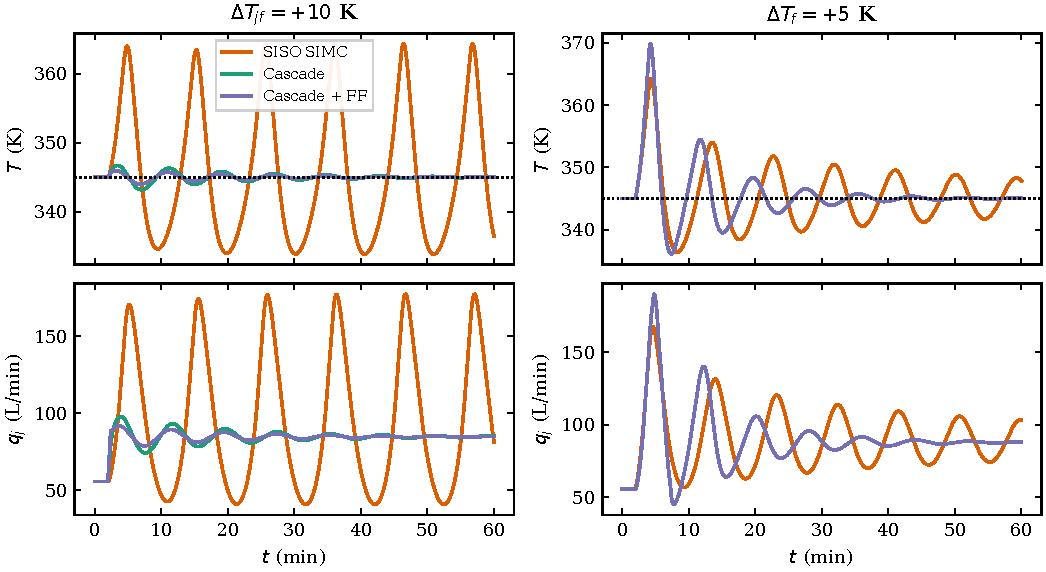
\includegraphics[width=\textwidth]{figures/fig3_saddle_shocks.pdf}
\caption{Reactor temperature (top) and coolant flow (bottom) at the saddle after a $+10$~K coolant supply shock (left) and a $+5$~K feed temperature shock (right) at $t=\tShock$~min. Dotted line: setpoint $\TSad$~K. In the right column the two cascade curves coincide because the feedforward does not measure $T_f$.}
\label{fig:shocks}
\end{figure*}

\paragraph{Coolant supply shock.} The single loop does not return to the setpoint. After the shock it enters a sustained oscillation with a peak deviation of $\peakTjfSiso$~K and a peak-to-peak amplitude of $\ptpTjfSiso$~K at the end of the run, and the valve travels $\tvTjfSiso$~L/min. The oscillation is not a slow transient. At the post-shock equilibrium ($T_{jf}=310$~K, $q_j=\qjShockTjf$~L/min) the jacket is closer to the supply temperature, the actuator gain drops to $b_3=\bThreeShockTjf$~K/L, and the linearized single loop has spectral abscissa $+\absShockTjfSiso$~min$^{-1}$: the shock moved the reactor to a point that the SISO gains no longer stabilize, and the bounded oscillation is the limit cycle of the nonlinear loop around an unstable closed-loop equilibrium. The same gains in the cascade give $\absShockTjfCascade$~min$^{-1}$ at that point. The cascade keeps the reactor within $\peakTjfCascade$~K of the setpoint and reduces the IAE by $\iaeRedTjf\%$ with less than a tenth of the valve travel. Here the classical argument for cascade control \cite{shinskey1996process,seborg2010process}, that the slave loop removes utility disturbances before they reach the reactor, holds in its strongest form: the disturbance enters the jacket balance, which is exactly the channel the slave controls. Feedforward from $T_{jf}$ through Eq.~\eqref{eq:ff} cuts the IAE by a further $\iaeRedFF\%$ and the peak deviation to $\peakTjfCascadeff$~K, because the slave bias jumps to the new equilibrium flow at the instant of the shock.

\paragraph{Feed temperature shock.} The feed shock enters the reactor energy balance directly, upstream of nothing the slave can measure. Both architectures now see a large transient: the peak deviation is $\peakTfSiso$~K for the single loop and $\peakTfCascade$~K for the cascade. The cascade still settles (peak-to-peak $\ptpTfCascade$~K over the last 20~min, linear spectral abscissa $\absShockTfCascade$~min$^{-1}$ at the post-shock equilibrium) and reduces the IAE by $\iaeRedTf\%$, whereas the single loop is still oscillating with $\ptpTfSiso$~K peak to peak after $\horizonShock$~min: its post-shock equilibrium is stable but barely ($\absShockTfSiso$~min$^{-1}$). The larger cascade peak follows from its master design: $\tau_{c1}=\theta_1$ is the default SIMC choice, not a tightened one, and the master integral time is short compared with the reactor response. As expected, the feedforward of Eq.~\eqref{eq:ff} does nothing here, and the two cascade rows coincide.

Taken together, the shocks show that at an unstable operating point the value of the cascade is not only faster disturbance rejection. The slave loop changes the plant seen by the master from unstable to stable (Section~\ref{subsec:cascade_design}), so the master can be tuned with the default SIMC rule and still keeps a stability margin when the operating point moves; the single loop, whose admissible $\tau_c$ interval is narrow (Table~\ref{tab:simc_sweep}), loses it after a moderate utility disturbance.

\subsection{Continuous fouling}
\label{subsec:res_fouling}
Table~\ref{tab:fouling} and Fig.~\ref{fig:fouling} report the fouling runs. The two operating points behave in qualitatively different ways.

\begin{table*}[t]
\centering
\footnotesize
\caption{Continuous fouling $d(UA)/dt=-\kappa_{\mathrm{foul}} r_A (UA-UA_{\min})$ with $\kappa_{\mathrm{foul}}=0.1$ L/mol and $UA_{\min}=0.30\,UA_0$. $t_{\mathrm{pred}}$: quasi-steady prediction (Eq.~\eqref{eq:t_pred}); $t_{\mathrm{sat}}$: first $q_j=u_{\max}$; $t_{\mathrm{runaway}}$: first $T-T_{sp}>5$ K.}
\label{tab:fouling}
\resizebox{\ifdim\width>\textwidth\textwidth\else\width\fi}{!}{%
\begin{tabular}{lcccccc}
\toprule
Point & Architecture & $t_{\mathrm{pred}}$ (min) & $t_{\mathrm{sat}}$ (min) & $UA(t_{\mathrm{sat}})/UA_0$ (\%) & $t_{\mathrm{runaway}}$ (min) & $T(80$ min) (K) \\
\midrule
Nominal & SISO SIMC & 8.92 & 10.02 & 57.0 & 13.18 & 416.40 \\
Nominal & Cascade & 8.92 & 9.26 & 59.0 & 13.18 & 416.40 \\
Saddle & SISO SIMC & 46.36 & 32.32 & 44.8 & 28.06 & 387.87 \\
Saddle & Cascade & 46.36 & 33.06 & 43.3 & 4.06 & 387.88 \\
\bottomrule
\end{tabular}%
}
\end{table*}


\begin{figure*}[t]
\centering
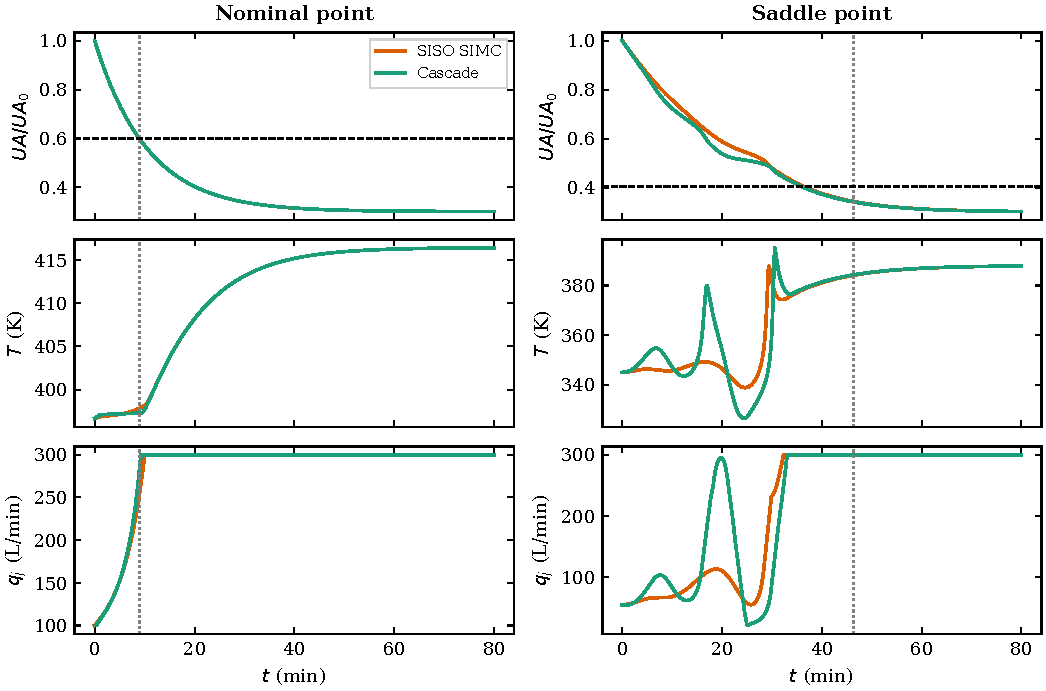
\includegraphics[width=\textwidth]{figures/fig4_fouling_runaway.pdf}
\caption{Continuous fouling at the nominal point (left) and at the saddle (right): heat-transfer capacity, reactor temperature and coolant flow. Dashed line: $UA_{\mathrm{crit}}$ from Eq.~\eqref{eq:ua_crit}; dotted line: $t_{\mathrm{pred}}$ from Eq.~\eqref{eq:t_pred}.}
\label{fig:fouling}
\end{figure*}

\paragraph{Nominal point: the thermodynamic limit is the binding one.} Both controllers hold the temperature while the valve opens, and the valve reaches $u_{\max}$ at $t_{\mathrm{sat}}=\tsatNomCascade$~min (cascade) and $\tsatNomSiso$~min (single loop), against $t_{\mathrm{pred}}=\tpredNom$~min from Eq.~\eqref{eq:t_pred}. The heat-transfer capacity at saturation, $\uaSatNomCascade\%$ and $\uaSatNomSiso\%$ of $UA_0$, is just below the $\fcritNom\%$ of Eq.~\eqref{eq:ua_crit}; the small delay is the tracking lag of each loop, larger for the slower single loop. After saturation the temperature leaves the setpoint ($t_{\mathrm{runaway}}=\trunNomCascade$~min for both) and climbs smoothly to $\TendNomCascade$~K, the stable equilibrium of the fouled reactor with the valve fully open. Because the nominal heat balance has a single root, there is no jump: the loss of regulation is a drift along the only branch, and its onset is predicted by a steady-state calculation.

\paragraph{Saddle: the loops fail long before the cooling capacity does.} At the saddle the quasi-steady prediction is $t_{\mathrm{pred}}=\tpredSad$~min, but neither loop gets there. The cascade first exceeds the $\bandRun$~K band at $\trunSadCascade$~min and the single loop at $\trunSadSiso$~min; both develop growing oscillations, the valve saturates during an excursion ($t_{\mathrm{sat}}=\tsatSadCascade$ and $\tsatSadSiso$~min), and the reactor ignites to the hot branch, ending at $\TendSadCascade$~K. The capacity at the moment of saturation, $\uaSatSadCascade\%$ and $\uaSatSadSiso\%$, is still above the critical $\fcritSad\%$: the valve did not saturate because the reactor needed more cooling than it could deliver, but because the loop had already become oscillatory.

\begin{figure}[t]
\centering
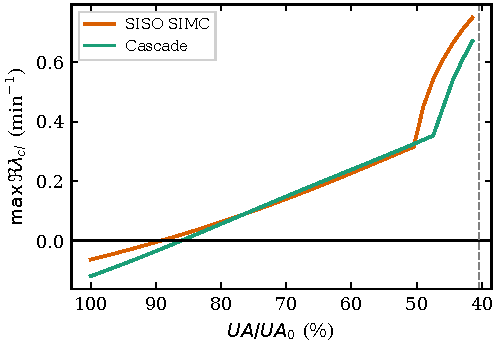
\includegraphics[width=\columnwidth]{figures/fig5_frozen_ua_stability.pdf}
\caption{Spectral abscissa of the linearized closed loop at the saddle for frozen values of $UA$, with gains tuned at $UA_0$. Dashed line: $UA_{\mathrm{crit}}$. Fixed-gain loops become unstable where the curves cross zero.}
\label{fig:frozen}
\end{figure}

Figure~\ref{fig:frozen} explains the mechanism. With gains fixed at their clean-jacket values, the linearized loops become unstable at $UA=\fstabSiso\%$ (single loop) and $\fstabCascade\%$ (cascade) of $UA_0$, where the equilibrium flows are only $\qstabSiso$ and $\qstabCascade$~L/min, far from the $\umax$~L/min of the valve. Fouling lowers the jacket temperature needed to hold the setpoint, which shrinks the actuator gain $b_3$ by a factor $\bThreeRatio$ between $UA_0$ and $UA_{\mathrm{crit}}$. For a controller that must keep $K_ck>1$ to hold an unstable pole (Section~\ref{subsec:siso_design}), losing actuator gain is losing stability. The cascade does not escape this: its slave loop acts on the same channel $b_3$, and once the slave is too weak the jacket coupling that it was cutting returns. In the fouling runs the cascade leaves the band earlier than the single loop most likely because the fast decline of $UA$ at the chosen $\kappa_{\mathrm{foul}}$ excites its less damped closed loop; the frozen-fouling boundary of Fig.~\ref{fig:frozen}, which does not depend on $\kappa_{\mathrm{foul}}$, shows that the two architectures lose the saddle at similar capacities.

The practical reading is that, on an open-loop unstable operating point, the controllability margin against fouling is not $UA_0-UA_{\mathrm{crit}}$ but $UA_0-UA_{\mathrm{stab}}$, and that the second is set by the controller rather than by the heat exchanger. Recovering the thermodynamic margin requires adapting the gain to the actuator effectiveness, for example by scheduling the slave gain on $1/(\bar T_j-T_{jf})$, which follows directly from Eq.~\eqref{eq:jacobian}; this is not tested here.

\subsection{Limitations}
The results rest on one reactor model with lumped, constant physical properties and perfect mixing. The saddle exists only with a feed cooled to $\TfSad$~K, a modification of the benchmark that we introduced because the nominal configuration has no unstable steady state; conclusions about the saddle should not be transferred to the nominal configuration, and the reverse. The fouling law of Eq.~\eqref{eq:fouling} is phenomenological and its rate constant is a scenario parameter chosen to keep the simulations short; only ratios to Eq.~\eqref{eq:t_pred} and the frozen-fouling boundaries are independent of it. Measurements are noise free, the valve has no stiction, and the controllers are PI only; derivative action, gain scheduling and model predictive control were not evaluated on the saddle. The stability statements are local, based on the Jacobian, and are confirmed but not proven globally by the nonlinear simulations.

\section{Conclusions}
\label{sec:conclusion}

The controllability of an exothermic CSTR with a dynamic jacket, a rate-limited coolant valve and a fouling heat exchanger was examined by separating three limits: open-loop instability, actuator authority and cooling capacity. The main findings are the following.
\begin{enumerate}
    \item The benchmark reactor has a single, stable steady state for every admissible coolant flow at its nominal feed temperature. An open-loop unstable saddle at $\TSad$~K, with $\lambda_1=+\lamASad$~min$^{-1}$, exists only when the feed is cooled to $\TfSad$~K. Claims of a metastable unstable window must be checked against the steady-state branches of the actual parameter set.
    \item For the unstable reduced model, the bound $\tau_c<\tau_u-\theta$ is exactly the condition $K_ck>1$ on the static loop gain; it is necessary, and for proportional control of this reactor it was also sufficient over the tested range. With the SIMC integral time the stabilizing interval shrinks to $\tau_c<\tcMaxPI$~min, and the default $\tau_c=\theta$ is unstable.
    \item Tight jacket regulation removes the instability: the concentration--temperature sub-block $\mathbf{A}_{12}$ is stable at the saddle, so the master loop of a cascade regulates a stable plant. The open-loop gain ratio overestimates the master gain by $\gainErrNom\%$ at the stable nominal point and has the wrong sign at the saddle; Eq.~\eqref{eq:k1_exact} gives the exact value.
    \item Against a $+10$~K coolant supply shock the cascade reduces the IAE by $\iaeRedTjf\%$ relative to the single loop, which falls into a limit cycle, and static feedforward from $T_{jf}$ removes a further $\iaeRedFF\%$. Against a feed temperature shock the cascade advantage is smaller ($\iaeRedTf\%$) and feedforward from $T_{jf}$ is ineffective.
    \item Under reaction-driven fouling the nominal point fails at the thermodynamic limit, $UA_{\mathrm{crit}}=\fcritNom\%\,UA_0$, at a time predicted by Eq.~\eqref{eq:t_pred}; at $55\%\,UA$ the heat generated at the setpoint exceeds the maximum removal for any control law. At the saddle, fixed-gain loops are lost at $\fstabCascade$--$\fstabSiso\%\,UA_0$, far above $UA_{\mathrm{crit}}=\fcritSad\%$, because fouling shrinks the actuator gain of the coolant valve.
\end{enumerate}
The last point is the one with the most direct consequence for operation: on an open-loop unstable branch, the margin against fouling is set by the controller and not by the heat exchanger. Gain scheduling on the jacket-to-supply temperature difference, adaptive or predictive control with an estimated heat-transfer capacity, and an experimental check of the fouling law are the natural next steps.


{\sloppy\printcredits}

\section*{Declaration of competing interest}
The authors declare that they have no known competing financial interests or personal relationships that could have appeared to influence the work reported in this paper.

\section*{Data availability}
{\sloppy All simulation code, campaign scripts, and data trajectories are openly accessible in the official project repository: \url{https://github.com/Marques-svnt/IC-CSTR-Control-Benchmark}.\par}

\bibliographystyle{elsarticle-num}
\bibliography{references}

\end{document}
